
\documentclass{article} % For LaTeX2e
\usepackage{iclr2025_conference,times}

% Optional math commands from https://github.com/goodfeli/dlbook_notation.
\input{math_commands.tex}

\usepackage{hyperref}
\usepackage{url}
\usepackage{graphicx}
\usepackage{booktabs}
\usepackage{lineno}
% \linenumbers

\title{扩散模型是实时游戏引擎}

\author{Dani Valevski\thanks{共同贡献。} \\
Google Research \\
daniv@google.com \\
\And
Yaniv Leviathan\footnotemark[1] \\
Google Research \\
leviathan@google.com \\
\And
Moab Arar\footnotemark[1] \\
Tel Aviv University\thanks{该工作完成于 Google Research 任职期间。} \\
moab.arar@gmail.com \\
\And
Shlomi Fruchter\footnotemark[1] \\
Google DeepMind \\
shlomif@google.com \\
}

\newcommand{\fix}{\marginpar{FIX}}
\newcommand{\new}{\marginpar{NEW}}

\iclrfinalcopy % Uncomment for camera-ready version, but NOT for submission.


% Chinese translation support
\usepackage{xeCJK}
\setCJKmainfont{FandolSong-Regular.otf}[ItalicFont=FandolKai-Regular.otf]
\setCJKsansfont{FandolHei-Regular.otf}
\setCJKmonofont{FandolFang-Regular.otf}
\XeTeXlinebreaklocale "zh"
\XeTeXlinebreakskip = 0pt plus 1pt
\renewcommand{\abstractname}{摘要}
\renewcommand{\figurename}{图}
\renewcommand{\tablename}{表}
\renewcommand{\refname}{参考文献}
\renewcommand{\contentsname}{目录}
\makeatletter
\AtBeginDocument{%
  \@ifundefined{crefname}{}{%
    \crefname{figure}{图}{图}%
    \Crefname{figure}{图}{图}%
    \crefname{table}{表}{表}%
    \Crefname{table}{表}{表}%
    \crefname{section}{节}{节}%
    \Crefname{section}{节}{节}%
    \crefname{appendix}{附录}{附录}%
    \Crefname{appendix}{附录}{附录}%
    \crefname{algocf}{算法}{算法}%
    \Crefname{algocf}{算法}{算法}%
  }%
  \@ifundefined{SetAlgorithmName}{}{\SetAlgorithmName{算法}{算法}{算法列表}}%
}
\makeatother
\raggedbottom

\begin{document}

\maketitle


\begin{abstract}
\vspace{-0.05in}
本文提出 \emph{GameNGen}，这是一个完全由神经模型驱动的游戏引擎，能够在复杂环境中以较高质量进行长轨迹实时交互。以经典游戏 DOOM 为训练对象时，GameNGen 从游戏轨迹中学习玩法，并生成一个可玩的环境，用于交互式模拟新的轨迹。\emph{GameNGen} 在单个 TPU 上以 20 FPS 运行，并能在数分钟的连续游玩中保持稳定。下一帧预测达到 29.4 PSNR，接近有损 JPEG 压缩的质量。即使经过 5 分钟自回归生成，人类评分者区分真实游戏片段和模拟片段的准确率也只略高于随机猜测。
GameNGen 的训练分为两个阶段：(1) 训练一个 RL 智能体玩游戏，并记录其训练过程中的轨迹；(2) 训练扩散模型，在给定历史帧和动作序列的条件下生成下一帧。条件噪声增强有助于长轨迹自回归生成的稳定性，解码器微调则提升了视觉细节和文本区域的保真度。
\end{abstract}


\begin{figure}[ht]
    \centering
    \vspace{-0.1in}
    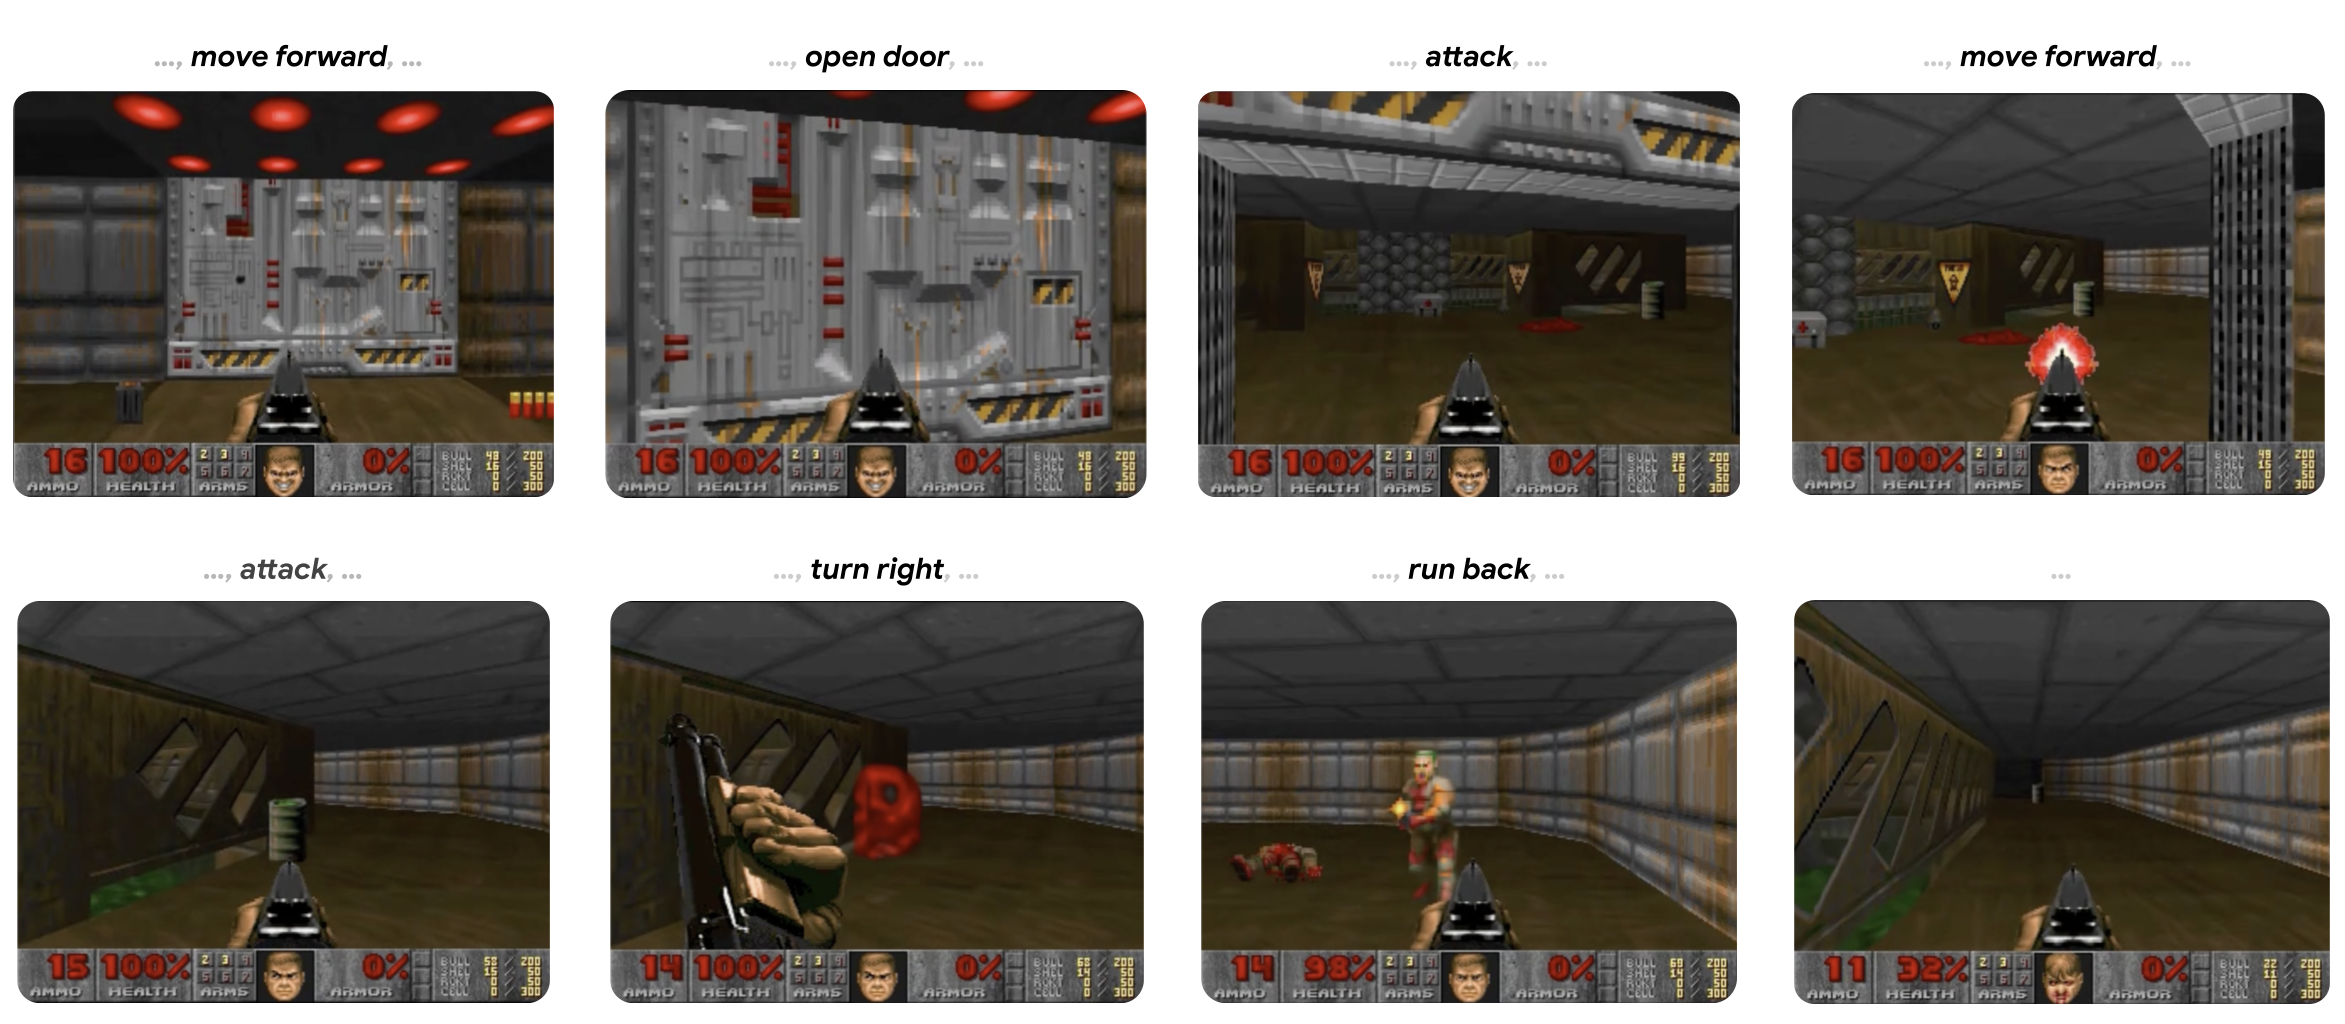
\includegraphics[width={\textwidth}]{figures/teaser.png}
    \caption{人类玩家正在通过 \textbf{GameNGen} 游玩 DOOM。多人分钟级实时游玩视频见 \url{https://gamengen.github.io}。}
    \label{fig:teaser}
    \vspace{-0.05in}
\end{figure}


\section{导言}

计算机游戏通常是人工编写的软件系统，其核心是一个 \emph{game loop}：先根据用户输入更新游戏状态，再将游戏状态渲染为屏幕像素。这个循环以较高帧率运行，给玩家造成一个可交互虚拟世界的体验。传统游戏循环运行在标准计算机上。虽然人们曾多次尝试在特殊硬件上运行游戏，例如经典游戏 DOOM 曾被移植到厨房电器、跑步机、相机以及 Minecraft 内部\footnote{见 \url{https://www.reddit.com/r/itrunsdoom/}}，但这些硬件本质上仍是在模拟人工编写的游戏软件。尽管游戏引擎之间差异很大，游戏状态更新和渲染逻辑仍主要由人工编程或配置的规则组成。

近年来，生成模型在以文本、图像等多模态输入为条件生成图像和视频方面取得了进展。扩散模型已经成为媒体生成，也就是非语言生成任务中的主流方法，代表工作包括 DALL-E~\citep{ramesh2022hierarchical}、Stable Diffusion~\citep{rombach2022high} 和 Sora~\citep{videoworldsimulators2024}。从表面看，模拟电子游戏中的交互世界似乎接近视频生成；但 \textit{交互式} 世界模拟并不只是高速视频生成。它必须在生成过程中持续接收动作流作为条件，这会打破现有扩散模型架构的一些假设。特别是，模型需要自回归地生成帧，而这种设置容易不稳定，并导致采样轨迹发散（见第~\ref{sec:mitigating ar noise} 节）。

已有一些重要工作尝试用神经模型模拟交互式电子游戏~\citep{ha2018worldmodels,Kim2020_GameGan,bruce2024genie}（见第~\ref{related_work} 节）。不过，这些方法通常会受限于可模拟游戏的复杂度、模拟速度、长时间稳定性或视觉质量（见图~\ref{fig:comp_with_prev_sota}）。
因此,自然要问:

\textit{一个在实时运行的神经模型能否以高品质模拟一个复杂的游戏?}

本文给出的答案是肯定的。我们展示了一个复杂电子游戏，即经典 DOOM，可以由神经网络实时运行。该神经网络是基于开源 Stable Diffusion v1.4~\citep{rombach2022high} 改造得到的模型，并能达到接近原游戏的视觉质量。虽然它不是精确模拟器（局限见第~\ref{sec:discussion} 节），但模型能够完成复杂的游戏状态更新，例如统计生命值和弹药、攻击敌人、破坏物体、开门，并在长轨迹中维持游戏状态。

本文的核心贡献是证明：复杂电子游戏（DOOM）可以由神经网络在单个 TPU 上以较高质量实时模拟。论文给出具体架构和技术经验，包括：(1) 通过噪声增强，将文本到图像扩散模型改造成稳定的自回归模型；(2) 通过微调潜在解码器，使视觉质量接近原游戏；(3) 通过 RL 智能体从现有游戏环境中大规模收集训练数据。

更广义地说，本文表明在现有硬件上实时模拟复杂游戏是可行的。这回答了通向新型游戏引擎范式中的一个关键问题：未来游戏可能像近年的图像和视频一样，由神经模型自动生成。当然，更大的问题仍未解决，例如如何利用人类输入创造全新游戏，而不只是模拟已有游戏。附录~\ref{appendix:new paradigm} 对这一方向作了进一步讨论。

\begin{figure}[ht]
    \centering
    \vspace{-0.1in}
    \includegraphics[width=\textwidth]{figures/compare_to_sota.pdf}
    \caption{\textbf{GameNGen 与已有 DOOM 模拟方法对比}：World Models~\cite{ha2018worldmodels} 与 GameGAN~\cite{Kim2020_GameGan}。注意，不同方法使用的训练数据并不相同。} 
    % }
    \label{fig:comp_with_prev_sota}
    \vspace{-0.05in}
\end{figure}

\section{互动世界模拟}
\label{sec:interactive world sim}

一个 \emph{交互式环境} $\mathcal{E}$ 由潜在状态空间 $\mathcal{S}$、潜在状态对应的观测空间 $\mathcal{O}$、部分投影函数 $V:\mathcal{S} \to \mathcal{O}$、动作集合 $\mathcal{A}$ 以及转移概率函数 $p(s| a, s')$ 组成，其中 $s, s' \in \mathcal{S}, a \in \mathcal{A}$。

以 DOOM 为例，$\mathcal{S}$ 是程序的动态内存内容，$\mathcal{O}$ 是渲染到屏幕上的像素，$V$ 是游戏渲染逻辑，$\mathcal{A}$ 是按键集合，$p$ 是给定玩家输入后的程序逻辑，其中也包括可能的非确定性。

给定交互式环境 $\mathcal{E}$ 和初始状态 $s_0 \in \mathcal{S}$，\emph{交互式世界模拟} 可以表示为一个 \emph{模拟分布函数} $q(o_n| o_{<n}, a_{\le n})$，其中 $o_i \in \mathcal{O}, a_i \in \mathcal{A}$。
给定观测之间的距离度量 $D:\mathcal{O}\times\mathcal{O} \to \mathbb{R}$、策略 $\pi(a_n|o_{<n}, a_{<n})$，即根据历史动作和观测给出智能体动作分布的函数、初始状态分布 $S_0$ 和回合长度分布 $N_0$，交互式世界模拟的目标是最小化 $E(D(o_q^i, o_p^i))$。其中 $n \sim N_0$，$0 \le i \le n$，$o_q^i \sim q$，$o_p^i \sim V(p)$，二者分别是在执行策略 $\pi$ 时从模拟器和真实环境中采样得到的观测。需要注意的是，这些样本中的条件动作始终来自智能体与环境 $\mathcal{E}$ 的交互；条件观测则可以来自 $\mathcal{E}$（即 \emph{teacher forcing 目标}），也可以来自模拟器本身（即 \emph{自回归目标}）。

本文始终使用 teacher forcing 目标训练生成模型。给定模拟分布函数 $q$ 后，可以通过自回归采样观测来模拟环境 $\mathcal{E}$。


\section{GameNGen}
\label{sec:method}

GameNGen（读作 “game engine”）是在第~\ref{sec:interactive world sim} 节设定下学习游戏模拟的生成式扩散模型。为按 teacher forcing 目标大规模收集训练数据，本文先训练一个独立模型与环境交互。智能体模型和生成模型按顺序训练：智能体训练过程中产生的全部动作与观测轨迹 $\mathcal{T}_{agent}$ 被保留下来，作为第二阶段生成模型的训练数据集。整体流程见图~\ref{fig:Overview}。

\begin{figure}
    \centering
    \includegraphics[width=0.99\linewidth]{figures/Architecture_08_27_b.pdf}
    \caption{方法概览（见第~\ref{sec:method} 节）。}
    \label{fig:Overview}
\end{figure}


\subsection{通过智能体游玩收集数据}
\label{agent-play}

最终目标是让人类玩家与模拟器交互，因此第~\ref{sec:interactive world sim} 节中的策略 $\pi$ 理想上应来自 \emph{人类游玩}。由于无法直接大规模采样人类游玩轨迹，本文先训练一个自动智能体来近似该策略。与通常追求最大游戏得分的 RL 设置不同，这里的目标是生成类似人类游玩的训练数据，或者至少覆盖足够多样的情境，以提高训练数据效率。为此，作者设计了一个简单奖励函数；这也是方法中唯一依赖具体环境的部分（见附录~\ref{appendix:reward}）。

作者记录智能体整个训练过程中的轨迹，因此数据覆盖从随机策略到较高技能水平的不同阶段。这组轨迹就是用于训练生成模型的 $\mathcal{T}_{agent}$ 数据集（见第~\ref{training-diffusion-model} 节）。

\subsection{训练生成式扩散模型}
\label{training-diffusion-model}

接下来训练一个以智能体轨迹 $\mathcal{T}_{agent}$（动作和观测）为条件的生成式扩散模型。

本文复用预训练文本到图像扩散模型 Stable Diffusion v1.4~\citep{rombach2022high}，使其预测游戏下一帧。模型 $f_{\theta}$ 以轨迹 $T \sim \mathcal{T}_{agent}$ 为条件，即以历史动作序列 $a_{<n}$ 和历史观测（帧）$o_{<n}$ 为条件，同时移除全部文本条件。
具体而言，对于动作条件（按键），作者学习一个动作嵌入 $A_{emb}$，将每个动作编码为一个 token，并用该动作序列替代原本来自文本的交叉注意力。对于观测条件（历史帧），作者用自动编码器 $\phi$ 将历史帧编码到潜在空间，并在潜在通道维度上与带噪 latent 拼接（见图~\ref{fig:Overview}）。作者也尝试过通过交叉注意力注入历史观测，但没有看到明显改进。

模型使用速度参数化的扩散损失训练~\citep{salimans2022progressivedistillationfastsampling}：

\begin{equation}
    \mathcal{L} = \mathbb{E}_{t,\epsilon,T} \left[ \| v(\epsilon, x_0, t) - v_{\theta'}(x_t, t, \{\phi(o_{i < n})\}, \{A_{emb}(a_{i < n})\}) \|_2^2 \right]
\end{equation}

其中$T = \{{o_{i \leq n}, a_{i \leq n}}\} \sim \mathcal{T}_{agent}$, $t \sim \mathcal{U}(0, 1)$, $\epsilon \sim \mathcal{N}(0, \mathbf{I})$, \mbox{$x_t = \sqrt{\bar{\alpha}_t} x_0 + \sqrt{1 - \bar{\alpha}_t} \epsilon$}, \mbox{$x_0 = \phi(o_n)$},
$v(\epsilon, x_0, t) = \sqrt{\bar{\alpha}_t} \epsilon - \sqrt{1 - \bar{\alpha}_t} x_0$,
其中 $v_{\theta'}$ 是模型 $f_{\theta}$ 的 v-prediction 输出。噪声调度 $\bar{\alpha}_t$ 为线性形式，与~\cite{rombach2022high} 类似。

\subsubsection{使用噪声增强缓解自回归漂移}
\label{sec:mitigating ar noise}

teacher forcing 训练与自回归采样之间存在分布偏移，会导致误差累积并使样本质量快速退化，如图~\ref{fig:noise_aug}（上）所示。为缓解自回归使用模型时产生的轨迹发散，作者在训练时对编码后的上下文帧加入不同强度的高斯噪声，并将噪声水平作为模型输入，这一做法参考了~\cite{ho2021cascaded}。具体而言，作者从 $[0, \alpha_{\max}]$ 中均匀采样噪声水平 $\alpha$，将其离散化，并为每个 bucket 学习一个嵌入（见图~\ref{fig:Overview}）。这样网络可以校正从过去帧中采样得到的信息，对长时间保持帧质量很关键。推理时，加入的噪声水平可调；不过作者发现，即使推理时不额外加噪声，训练时使用该增强也能明显改善结果。第~\ref{noise-aug-abalation} 节对其影响做了消融。

\begin{figure}[t]
    \centering
    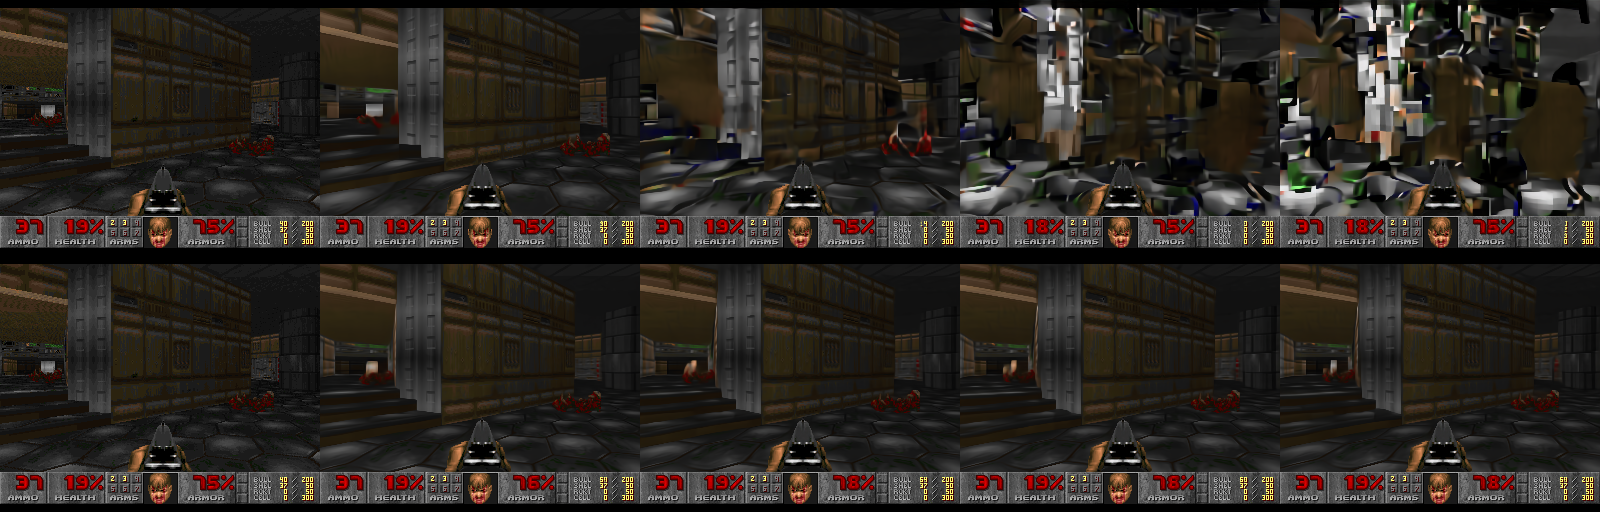
\includegraphics[width=1.0\textwidth]{figures/noise_aug_ablation_new.png}
    \caption{\textbf{自回归漂移。} 上：一个玩家不移动的简单轨迹，每 10 帧展示一次；生成质量在 20 到 30 步后迅速下降。下：使用噪声增强后，同一轨迹没有出现明显质量退化。}
    \label{fig:noise_aug}
\end{figure}

\subsubsection{潜在解码器微调}
\label{sec:autoencoder fine tuning}

Stable Diffusion v1.4 的预训练自动编码器会将 $8\times8$ 像素 patch 压缩为 4 个潜在通道。直接用于游戏帧预测时，它会产生明显伪影，影响小细节，尤其是底部 HUD（heads-up display）区域。为在保留预训练知识的同时提升图像质量，作者只训练潜在自动编码器的解码器，并用目标帧像素上的 MSE 损失进行监督。
需要注意的是，该微调过程与 U-Net 微调完全分离；自回归生成本身不受该步骤影响，因为模型只在 latent 上自回归条件化，而不是在像素上条件化。附录~\ref{appendix:fine-tune-vae} 展示了微调和不微调自动编码器时的生成示例。

\subsection{推理}
\label{sec:inference}

\subsubsection{设置}

推理时使用 DDIM 采样~\citep{song2022denoisingdiffusionimplicitmodels}。作者只对历史观测条件 $o_{<n}$ 使用 classifier-free guidance~\citep{ho2022classifierfreediffusionguidance}；对历史动作条件 $a_{<n}$ 使用 guidance 没有带来质量提升。guidance 权重设为较小的 1.5，因为更大的权重会产生伪影，并在自回归采样中进一步累积。

\subsubsection{Denoiser 采样步骤}
推理期间需要运行 U-Net denoiser 若干步，并运行自动编码器。在作者的硬件配置中，单个 TPU-v5 上一次 denoiser 步骤和一次自动编码器评估各需要约 10ms。如果只使用一个 denoiser 步骤，理论最小总延迟约为每帧 20ms，即 50 FPS。
通常，Stable Diffusion 这类生成式扩散模型无法用单次去噪得到高质量结果，而需要数十个采样步骤。作者发现，在 DOOM 模拟中，仅使用 4 个 DDIM 采样步骤~\citep{song2020denoising} 即可稳定工作。与 20 步或更多采样步相比，4 步采样没有观察到明显质量退化（见表~\ref{table:diffusion_steps_quality} 和附录~\ref{appendix:ablate num sampling steps}）。
\begin{table}[h]
\caption{\textbf{不同采样步数下的生成。} 使用 PSNR 和 LPIPS 指标评价 GameNGen 在不同采样步数下的生成质量。“D”表示一步蒸馏模型。更多细节见附录~\ref{appendix:distillation}。}
\label{table:diffusion_steps_quality}
\centering
\vspace{0.05in}
\resizebox{0.40\textwidth}{!}{
\begin{tabular}{ccc}
\toprule
步骤 & PSNR$\uparrow$ & LPIPS$\downarrow$ \\
\midrule
D   &  $31.10 \pm 0.098$  &  $0.208 \pm 0.002$ \\ % SD: 2.27, 0.049
1   &  $25.47 \pm 0.098$  &  $0.255 \pm 0.002$ \\ % SD: 2.26, 0.043
2   &  $31.91 \pm 0.104$  &  $0.205 \pm 0.002$ \\ % SD: 2.39, 0.050
4   &  $32.58 \pm 0.108$  &  $0.198 \pm 0.002$ \\ % SD: 2.49, 0.049
8   &  $32.55 \pm 0.110$  &  $0.196 \pm 0.002$ \\ % SD: 2.53, 0.049
16  &  $32.44 \pm 0.110$  &  $0.196 \pm 0.002$ \\ % SD: 2.54, 0.048
32  &  $32.32 \pm 0.110$  &  $0.196 \pm 0.002$ \\ % SD: 2.54, 0.048
64  &  $32.19 \pm 0.110$  &  $0.197 \pm 0.002$ \\ % SD: 2.53, 0.048
\bottomrule
\end{tabular}
}
\end{table}
仅使用 4 个去噪步骤时，U-Net 总耗时约 40ms；加上自动编码器后，总推理耗时约 50ms，对应 20 FPS。作者认为，少量采样步对质量影响较小，可能来自两个因素：(1) 图像空间受游戏环境约束；(2) 历史帧提供了强条件。

由于单步采样会明显退化，作者还参考~\citep{yin2024onestep,wang2023prolificdreamer} 在单步设置下尝试模型蒸馏。蒸馏确实能提升单步模型质量，并使系统达到 50 FPS，但仍会牺牲一定模拟质量。因此，本文主方法采用不蒸馏的 4 步版本（见附录~\ref{appendix:distillation}）。%This is an interesting area for further research.


\section{实验设置}
\label{experimental_setup}

\subsection{智能体训练}
智能体使用 PPO~\citep{SchulmanWDRK17ppo} 训练，特征网络为一个简单 CNN，设置参考~\cite{Mnih2015HumanlevelCT}，并基于 Stable Baselines 3~\citep{stable-baselines3} 在 CPU 上训练。智能体输入包括降采样后的帧图像和游戏内地图，二者分辨率均为 $160\times120$。智能体还可以访问最近 32 个已执行动作。特征网络为每张图像计算 512 维表示，PPO 的 actor 和 critic 都是 2 层 MLP，输入为图像特征和历史动作序列的拼接。
作者使用 ViZDoom 环境训练智能体玩游戏~\citep{Wydmuch2019ViZdoom}。训练时并行运行 8 个游戏，每个 replay buffer 大小为 512，折扣因子 $\gamma=0.99$，熵系数为 $0.1$。每次迭代中，网络以 batch size 64 训练 10 个 epoch，学习率为 $10^{-4}$。总训练量为 50M 环境步。

\subsection{生成模型训练}
所有模拟模型都从 Stable Diffusion 1.4 的预训练 checkpoint 初始化，并解冻全部 U-Net 参数。训练使用 batch size 128、常数学习率 $2\times10^{-5}$、无权重衰减的 Adafactor 优化器~\citep{Shazeer2018adafactor}，以及 1.0 的梯度裁剪。为支持推理时的 CFG，上下文帧条件以 0.1 的概率被 drop。模型在 128 个 TPU-v5e 设备上做数据并行训练。除非另有说明，论文所有结果均来自训练 700k 步后的模型。
噪声增强（第~\ref{sec:mitigating ar noise} 节）使用最大噪声水平 0.7，并划分为 10 个 embedding bucket。潜在解码器优化时 batch size 为 2,048，其余训练参数与 denoiser 相同。
训练数据使用智能体在 RL 训练和评估期间记录轨迹中的随机子集，共 70M 个样本；更小数据规模的结果见附录~\ref{appendix-dataset-size}。所有图像帧在训练、推理和条件化时均为 $320\times240$，并填充到 $320\times256$。上下文长度为 64，也就是模型会看到自己最近 64 个预测帧以及最近 64 个动作。

\section{结果}
\label{sec:results}

\subsection{模拟质量}
\label{sec:sim quality}

整体来看，本文方法在长轨迹上的图像质量接近原游戏。对于短片段，人类评分者区分模拟和真实游戏的表现仅略高于随机猜测。

\textbf{图像质量。} 图像质量使用 LPIPS~\citep{zhang2018perceptual} 和 PSNR 衡量。评估采用第~\ref{sec:interactive world sim} 节中的 teacher forcing 设置：采样一个初始状态，并基于真实历史观测轨迹预测单帧。在来自 5 个不同关卡的 2048 条随机保留轨迹上，模型达到 $29.43$ PSNR 和 $0.249$ LPIPS。该 PSNR 接近质量参数为 20 到 30 的有损 JPEG 压缩~\citep{petric2018comparisoncsjpegterms}。图~\ref{fig:predcition_samples} 展示模型预测和对应真实值样本。

\begin{figure}[t]
    \centering
    \includegraphics[width=1.0\textwidth]{figures/image_quality.pdf}
    \caption{\textbf{模型预测与真实值。} 图中只展示历史观测上下文的最后 4 帧。}
    \label{fig:predcition_samples}
\end{figure}

\textbf{视频质量。} 视频质量使用第~\ref{sec:interactive world sim} 节的自回归设置评估：模型按照真实轨迹中的动作序列迭代采样帧，同时以自己的历史预测作为条件。自回归采样时，预测轨迹和真实轨迹通常会在若干步后发生偏离，主要原因是帧间运动速度的微小差异会逐步累积。因此，如图~\ref{fig:ar_eval} 所示，逐帧 PSNR 会下降，LPIPS 会上升。尽管如此，从内容和图像质量上看，预测轨迹仍与真实游戏相似，只是逐帧指标难以完整捕捉这种相似性。自回归生成样例见附录~\ref{appendix-samples}。

因此，作者进一步计算 FVD~\citep{UnterthinerSKMM19FVD}，用 512 条随机保留轨迹衡量预测轨迹分布与真实轨迹分布之间的距离。对于 16 帧（0.8 秒）模拟，模型 FVD 为 $114.02$；对于 32 帧（1.6 秒）模拟，FVD 为 $186.23$。

\textbf{人类评估。} 作为另一种模拟质量指标，作者向 10 名人类评分者展示 130 个随机短片段，片段长度为 1.6 秒或 3.2 秒，并将模拟片段与真实游戏并排展示（见附录~\ref{appendix:human eval} 的图~\ref{fig:eval tool}）。评分者在 1.6 秒和 3.2 秒片段中分别只有 58\% 和 60\% 的时间能选出真实游戏。为评估自回归误差累积的影响，作者还在模拟游玩 5 到 10 分钟后，额外生成 150 组 3 秒片段做并排比较。尽管自回归生成持续时间较长，评分者仍接近随机水平，仅在 50\% 的时间识别出真实游戏。
需要指出的是，熟悉模拟局限的作者通常能在几秒内识别真实游戏。更长的分钟级片段质量可参考补充材料视频。


\begin{figure}[t]
    \centering
    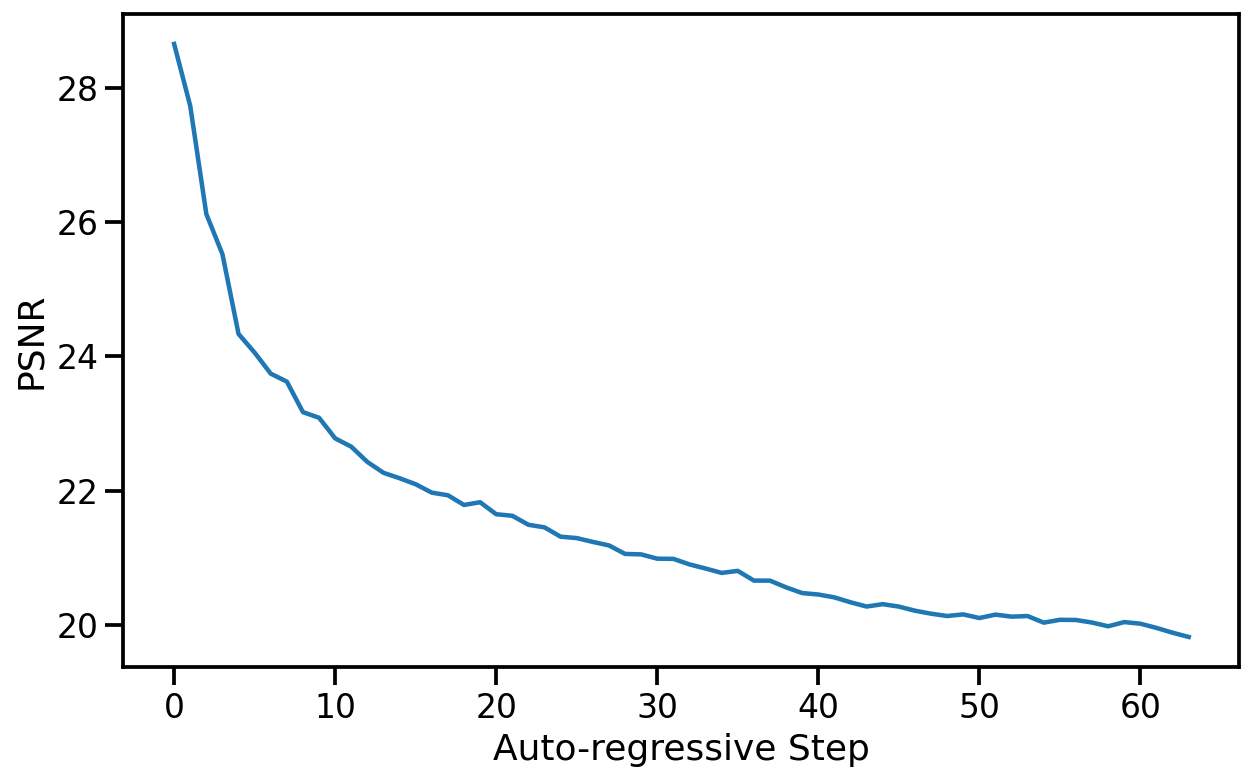
\includegraphics[width=0.4\textwidth]{figures/psnr_step_700k_08212004.png}
    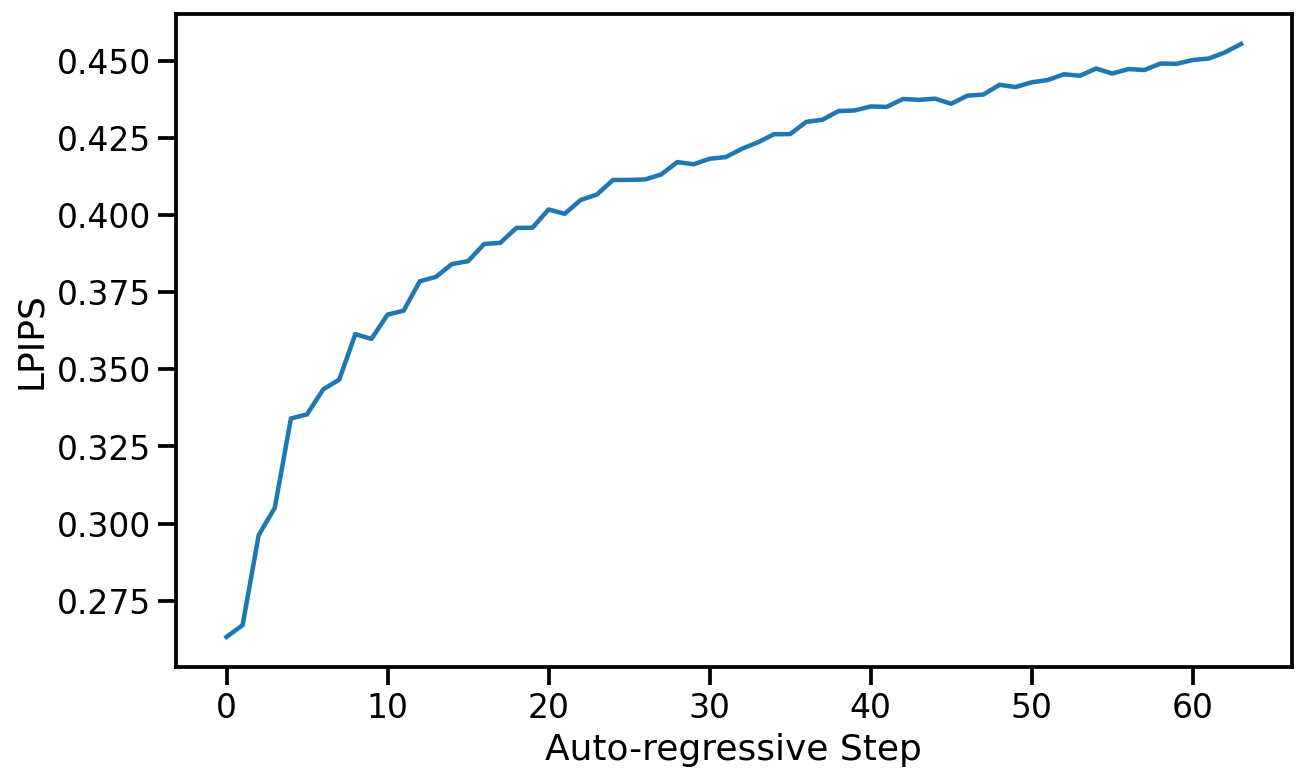
\includegraphics[width=0.4\textwidth]{figures/lpips_step_700k_08212004.png}
    \caption{\textbf{自回归评估。} 64 个自回归步骤上的 PSNR 和 LPIPS 指标。}
    \label{fig:ar_eval}
\end{figure}


\subsection{消融实验}

为评估方法各组成部分的重要性，作者从评估数据集中采样轨迹，并计算预测帧与真实帧之间的 LPIPS 和 PSNR。

\subsubsection{上下文长度}
\label{sec:context length}

作者通过训练不同历史观测数量 $N$ 的模型来评估上下文长度影响，其中 $N \in \{1, 2, 4, 8, 16, 32, 64\}$，本文主方法使用 $N=64$。改变 $N$ 会同时改变历史帧数和历史动作数。所有模型训练 200k 步，保持解码器冻结，并在 5 个关卡的测试轨迹上评估。结果见表~\ref{table:number_of_frames_ablation}。
如预期，生成质量随上下文长度增加而提升。提升在一开始较明显，例如从 1 帧增加到 2 帧；但很快接近平台期，继续增加上下文只带来较小收益。这一点值得注意，因为即使最大上下文长度也只覆盖略多于 3 秒历史，而论文在第~\ref{sec:discussion} 节观察到许多游戏状态可以保持更久。表~\ref{table:number_of_frames_ablation} 暗示，仅增加上下文长度可能不够，未来需要改进架构、训练方案，或更有效地选择历史帧作为条件。

\begin{table}[h]
\caption{\textbf{历史帧数量。} 使用来自 5 个关卡的 8912 个测试样本消融上下文历史帧数。更多历史帧通常会改善 PSNR 和 LPIPS。\label{table:number_of_frames_ablation}}
\centering
\vspace{0.05in}
\resizebox{0.5\textwidth}{!}{
\begin{tabular}{lcccc}
\toprule
历史上下文长度 & PSNR$\uparrow$ & LPIPS$\downarrow$ \\
\midrule
    64  &  $22.36 \pm 0.033$  &  $0.295 \pm 0.001$ \\ % SD: 1.59, 0.048
    32  &  $22.31 \pm 0.033$  &  $0.296 \pm 0.001$ \\ % SD: 1.58, 0.049
    16  &  $22.28 \pm 0.033$  &  $0.296 \pm 0.001$ \\ % SD: 1.59, 0.049
8  &  $22.26 \pm 0.033$  &  $0.296 \pm 0.001$ \\ % SD: 1.59, 0.049
4  &  $22.26 \pm 0.034$  &  $0.298 \pm 0.001$ \\ % SD: 1.64, 0.048
2  &  $22.03 \pm 0.037$  &  $0.304 \pm 0.001$ \\ % SD: 1.77, 0.050
1  &  $20.94 \pm 0.044$  &  $0.358 \pm 0.001$ \\ % SD: 2.14, 0.062
\bottomrule
\end{tabular}
}
\end{table}

\subsubsection{噪声增强}
\label{noise-aug-abalation}

为消融噪声增强的影响，作者训练了一个不使用额外噪声的模型。然后在 200k 训练步后，对标准噪声增强模型和无噪声增强模型进行自回归评估，并在 512 条随机保留轨迹上计算预测帧与真实帧之间的 PSNR 和 LPIPS。图~\ref{fig:noise_aug_abalation} 报告了最多 64 个自回归步骤中每一步的平均指标。

没有噪声增强时，LPIPS 相比标准模型迅速上升，PSNR 下降，说明模拟轨迹更快偏离真实轨迹。

\begin{figure}[h]
    \centering
    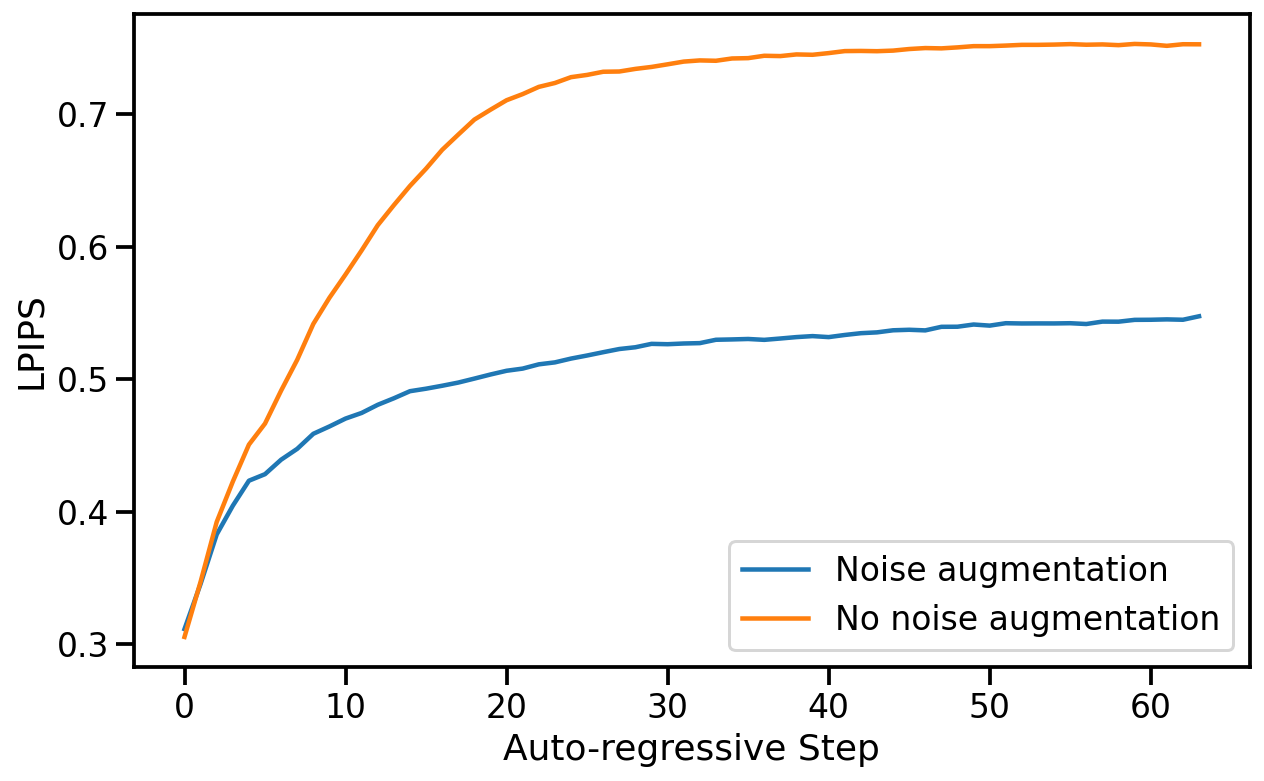
\includegraphics[width=0.45\textwidth]{figures/noise_aug_ablation_lpips_step_200k_08212024.png}
    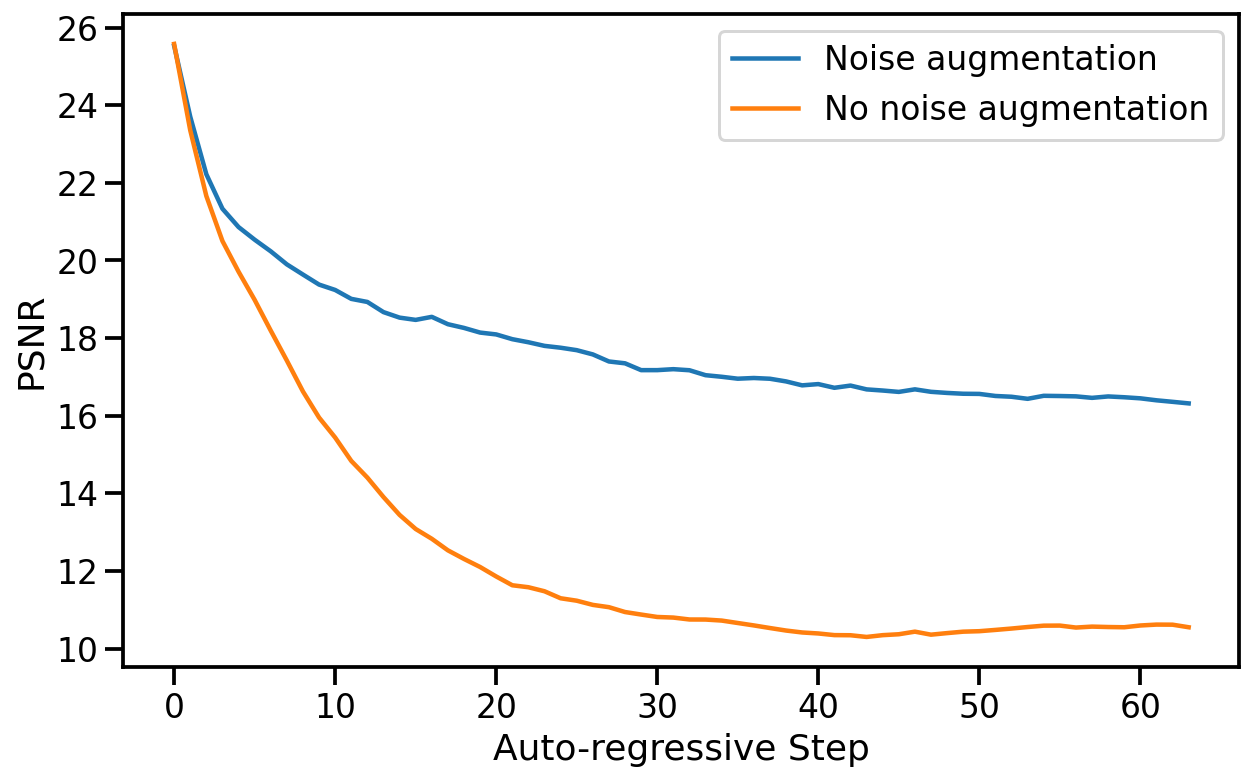
\includegraphics[width=0.45\textwidth]{figures/noise_aug_ablation_psnr_step_200k_08212024.png}
    \caption{\textbf{噪声增强的影响。} 曲线展示每个自回归步骤的平均 LPIPS（越低越好）和 PSNR（越高越好）。不使用噪声增强时，质量在 10 到 20 帧后迅速退化；噪声增强可以缓解这一问题。}
    \label{fig:noise_aug_abalation}
\end{figure}

\subsubsection{智能体播放}
\label{agent-play-ablation}

作者比较了用智能体生成数据训练和用随机策略生成数据训练的效果。随机策略按与观测无关的均匀类别分布采样动作。为比较两类数据集，作者分别训练两个模型及其解码器 700k 步，并在来自 5 个关卡的 2048 条人类游玩轨迹上评估。评估包括两种情况：在 64 帧真实历史上下文条件下预测第一帧，以及自回归生成 3 秒后的某一帧。

总体来看，用随机轨迹训练也能得到不错结果，但受限于随机策略的探索能力。单帧生成时，智能体数据只略好于随机数据，PSNR 分别为 25.06 和 24.42。自回归生成 3 秒后，差距扩大到 19.02 对 16.84。手动体验时，一些区域对两种模型都很容易，一些区域都很难，而在部分中等难度区域，智能体数据明显更好。作者据此按与游戏起点的距离将 456 个样本人工划分为 easy、medium、hard 三档。结果显示，在 easy 和 hard 集合上，智能体数据只略好于随机数据；在 medium 集合上，智能体数据优势更大（见表~\ref{table:difficulty_split_performance}）。单次人类游玩中的得分示例见附录~\ref{appendix:agent v random} 的图~\ref{fig:agent v random}。

\begin{table}[t]
\caption{\textbf{不同难度下的性能。} 比较使用智能体生成数据和随机生成数据训练的模型，在 easy、medium、hard 三个划分上的表现。easy 和 medium 各有 112 项，hard 有 232 项。指标在 3 秒后每条轨迹的单帧上计算。\label{table:difficulty_split_performance}}
\centering
\vspace{0.05in}
\resizebox{0.75\textwidth}{!}{
\begin{tabular}{lcccc}
\toprule
难度 & 数据生成策略 & PSNR$\uparrow$ & LPIPS$\downarrow$ \\
\midrule
Easy & 智能体 & $20.94 \pm 0.76$ & $0.48 \pm 0.01$ \\
        & 随机 & $20.20 \pm 0.83$ & $0.48 \pm 0.01$ \\
\midrule
Medium & 智能体 & $20.21 \pm 0.36$ & $0.50 \pm 0.01$ \\
        & 随机 & $16.50 \pm 0.41$ & $0.59 \pm 0.01$ \\
\midrule
Hard & 智能体 & $17.51 \pm 0.35$ & $0.60 \pm 0.01$ \\
        & 随机 & $15.39 \pm 0.43$ & $0.61 \pm 0.00$ \\
\bottomrule
\end{tabular}
}
\end{table}

% \section{Societal Impact}

\section{有关工作}
\label{related_work}

\textbf{游戏模拟与世界模型。} 一些工作尝试在动作输入条件下训练游戏模拟模型。\cite{yang2023learning} 构建了包含真实世界和模拟视频的多样化数据集，并训练扩散模型，在给定前一段视频和动作文本描述的条件下预测后续视频。\cite{menapace2021playablevideogeneration} 和 \cite{bruce2024genie} 关注从视频中无监督学习动作。\cite{Menapace_2024} 将文本提示转换为游戏状态，再使用 NeRF 将这些状态转换为 3D 表示。

另一条路线学习环境预测模型，并将其用于训练 RL 智能体。\cite{ha2018worldmodels} 训练变分自编码器~\citep{Kingma2014} 将游戏帧编码为潜在向量，再用 RNN 模拟 ViZDoom 环境；训练数据来自随机策略的 rollout，即随机选择动作。随后，控制器策略在这个“幻觉”环境中学习。\cite{hafner2020dreamer} 证明 RL 智能体可以完全在由学习型世界模型生成的潜在空间回合中训练。

与本文接近的还有 \cite{Kim2020_GameGan}，该工作使用 LSTM 架构建模世界状态，并结合卷积解码器生成输出帧，在对抗目标下联合训练。

\cite{yan2021videogpt} 将 decoder-only Transformer 架构用于视频生成，使用 VQ-VAE 学到的离散潜在空间，并展示其可用于 ViZDoom 模拟器上的动作条件视频生成。

\cite{gaia2023} 关注驾驶领域的动作条件世界建模问题。该方法使用多模态自回归 Transformer 作为世界模型，根据历史图像、文本和动作 token 预测潜在空间图像 token，再由扩散视频解码器将图像 token 转换为像素空间视频。模型在大规模真实驾驶数据上训练，包含 420M 张唯一图像。

最后，与本文同期，\cite{alonso2024diffusion} 训练了一个扩散世界模型，根据观测历史预测下一观测，并在 Atari 上迭代训练世界模型和 RL 模型。其后续版本还包含 Counter-Strike 的高分辨率模拟，训练数据为 95 小时人类游戏录像。

\textbf{自回归扩散模型。} 近期一些工作探索了扩散模型的自回归结构。\cite{chen2024diffusionforcingnexttokenprediction} 不同于传统扩散架构，它允许每个 token 在每个时间步具有自己的噪声水平，并在使用卷积 RNN 主干时报告了超过训练视野的视频生成稳定性提升。\cite{rollingdiffusion2024} 也通过滑动窗口去噪过程，为不同 token 设置可变噪声水平。这类方法对实时游戏模拟很有参考价值，本文将其留作后续工作。

\textbf{DOOM。} DOOM 于 1993 年发布，对游戏行业产生了重要影响。它引入了当时具有代表性的 3D 图形技术，成为第一人称射击类型的重要基础，并影响了大量后续游戏。DOOM 也被许多研究工作采用。它有开源实现，原生分辨率较低，小模型也有可能进行模拟；同时游戏逻辑又足够复杂，适合作为有挑战性的测试案例。最后，作者们年轻时也在这款游戏上投入了大量时间，因此选择 DOOM 作为实验对象相当自然。


\section{讨论情况}
\label{sec:discussion}

\textbf{总结。} 本文介绍了 \emph{GameNGen}，并证明神经模型可以以 20 FPS 进行较高质量的实时游戏模拟。

\textbf{局限性。} (1) GameNGen 的记忆长度有限。模型只能访问略多于 3 秒的历史，因此它能够在更长时间范围内维持许多游戏逻辑这一点值得注意（补充材料提供了分钟级游玩视频）。部分游戏状态会持续显示在屏幕像素中，例如弹药、生命值和可用武器等；模型也可能学习到较强启发式规则，从而做出有意义的泛化。例如，模型可以从渲染视图推断当前位置，也可能根据弹药和生命值估计某一区域敌人是否已被击败。不过，仍然容易构造出上下文长度不足的情形（见补充视频）。这些启发式也可能出错，例如如果玩家反复射击，GameNGen 可能会生成敌人，因为训练中的智能体通常会在敌人出现时射击。按现有架构继续增加上下文只带来有限收益（第~\ref{sec:context length} 节），短上下文仍是重要限制。
(2) 第二个限制是智能体行为与人类玩家行为之间仍有差异。例如，即使训练结束，智能体也没有探索游戏中的所有位置和交互，导致这些情形下模型可能出现错误行为（见补充视频）。
(3) 另一个限制是，GameNGen 还不能像传统游戏引擎那样方便地制作新游戏。它可以像传统游戏引擎一样交互式运行 game loop，即根据输入更新状态并渲染到屏幕；但多数游戏引擎还提供容易创建新游戏的能力，GameNGen 目前不具备这一点。

\textbf{未来工作。} 本文只在经典游戏 DOOM 上展示 GameNGen。未来可以在其他游戏，或者更一般的交互式软件系统上测试该方法。除 RL 智能体的奖励函数外，本文技术并不特定于 DOOM，作者计划在后续工作中进一步降低这一环境依赖。GameNGen 虽然能较准确地维持游戏状态，但仍不完美；更复杂的架构和训练方案可能有助于缓解上述问题。模型目前利用长记忆的能力有限，对更复杂游戏或软件而言，有效扩展记忆可能很关键。GameNGen 在 TPUv5 上可运行于 20 或 50 FPS\footnote{这比 DOOM 原版当年在部分作者的 80386 机器上运行还快。}，未来可继续探索更高帧率和消费级硬件部署。

\textbf{迈向交互式电子游戏的新范式。}
\label{appendix:new paradigm}
今天的电子游戏主要由人类编程。GameNGen 是一种新范式的概念验证：游戏可以被表示为神经模型权重，而不是代码行。它表明，存在某种架构和模型权重，使神经模型能够在现有硬件上交互式运行复杂游戏（DOOM）。
这一范式仍有许多问题，但可能带来新的开发方式。例如，游戏开发过程可能成本更低、门槛更低，用户可以通过文本描述或示例图像开发和编辑游戏。短期内，更现实的目标是为已有游戏创建修改或新行为。例如，可以尝试将一组帧转换成新的可玩关卡，或仅根据示例图像创建新角色，而无需手写代码（见附录~\ref{appendix-out-of-distribution}）。作者尚未系统探索这些方向，仍需要大量工作。

\section*{更大的影响}
\textbf{社会影响。} GameNGen 表明，神经网络可以实时模拟交互式游戏，为游戏开发提供新的可能性。与 LLM、文本到图像模型和文本到视频模型等生成技术类似，后续需要研究如何让用户和游戏开发者负责任地构建新体验。

\textbf{可复现性。} 作者在实现选择上优先考虑可复现性。基础模型采用相对较小且开源、开放权重的 Stable Diffusion 1.4，便于微调。游戏环境使用文档充分且开源的 VizDoom。论文还详细描述了训练参数和数据生成配置，并共享性能指标，作为后续工作的基线。

\section*{鸣谢}

作者感谢 Eyal Segalis、Eyal Molad、Matan Kalman、Nataniel Ruiz、Amir Hertz、Matan Cohen、Yossi Matias、Yael Pritch、Danny Lumen、Valerie Nygaard、Michelle Tadmor Ramanovich、Theta Labs、Google Research 团队以及作者家人提供的反馈、想法、建议和支持。

\section*{捐款}
Shlomi 和 Yaniv 提出了项目、方法和架构，开发了初始实现，并对实现和写作作出关键贡献。Dani 开发了最终代码库的大部分内容，调试了系统参数和细节，并加入自动编码器微调、智能体训练和蒸馏。Moab 主导了通过噪声增强实现自回归稳定性的工作，完成多项消融实验，并创建了人类游玩数据集。

\bibliography{iclr2025_conference}
\bibliographystyle{iclr2025_conference}

\clearpage

\newpage

\appendix
\section{附录}

\subsection{样本}
\label{appendix-samples}
图~\ref{fig:samples_1}, \ref{fig:samples_2}, \ref{fig:samples_3}, \ref{fig:samples_4} 给出 GameNGen 的若干生成样本。
\begin{figure}[h]
    \centering
    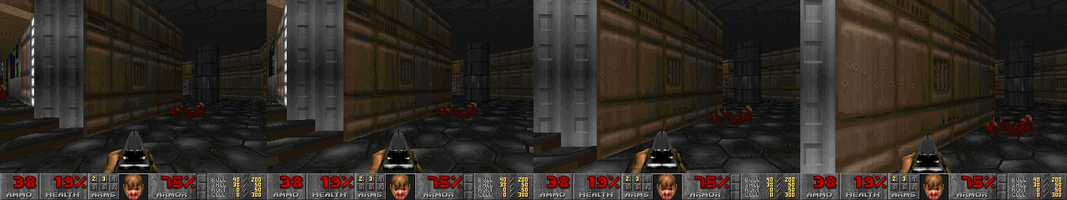
\includegraphics[width=1.0\textwidth]{figures/samples/context_1.png}
    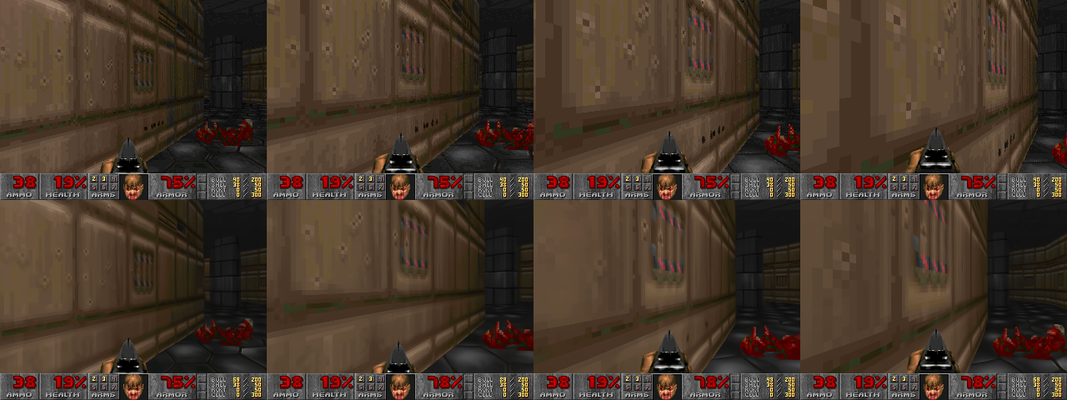
\includegraphics[width=1.0\textwidth]{figures/samples/gt_vs_predicted_1.png}
    \caption{\textbf{模拟模型的自回归评估：样本 \#1。} 上行：上下文帧；中行：真实帧；下行：模型预测。}
    \label{fig:samples_1}
\end{figure}

\begin{figure}[h]
    \centering
    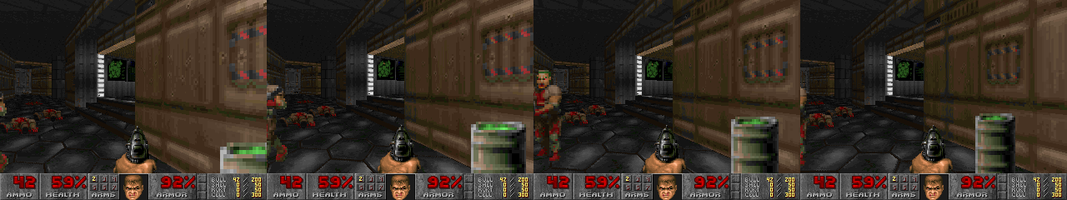
\includegraphics[width=1.0\textwidth]{figures/samples/context_3.png}
    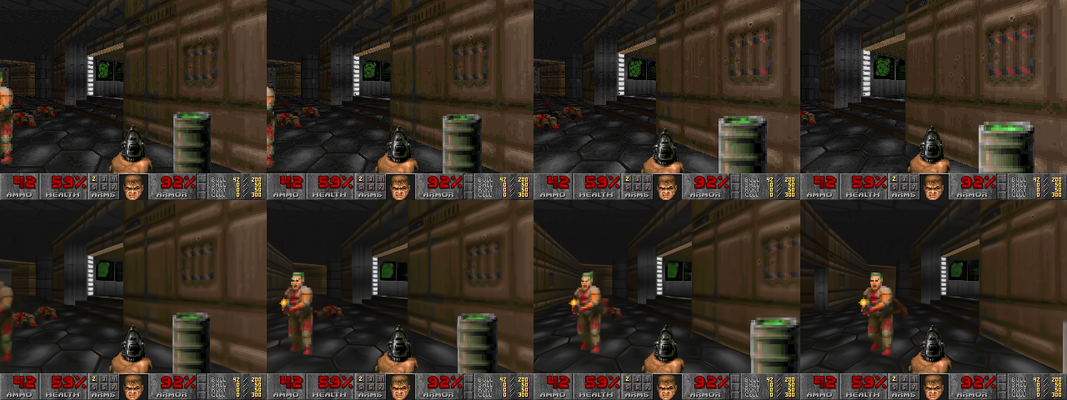
\includegraphics[width=1.0\textwidth]{figures/samples/gt_vs_predicted_3.png}
    \caption{\textbf{模拟模型的自回归评估：样本 \#2。} 上行：上下文帧；中行：真实帧；下行：模型预测。}
    \label{fig:samples_2}
\end{figure}

\begin{figure}[h]
    \centering
    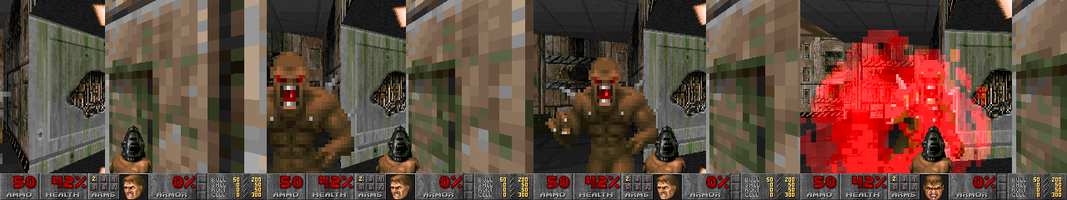
\includegraphics[width=1.0\textwidth]{figures/samples/context_5.png}
    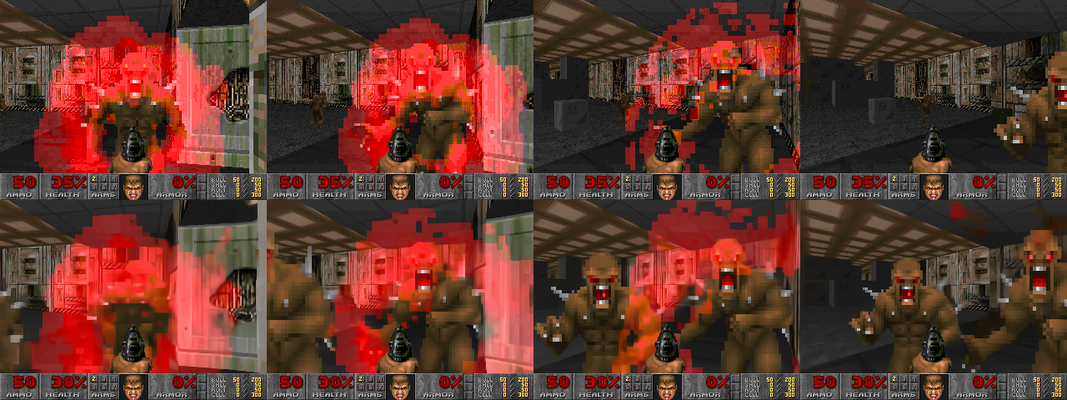
\includegraphics[width=1.0\textwidth]{figures/samples/gt_vs_prediction_5.png}
    \caption{\textbf{模拟模型的自回归评估：样本 \#3。} 上行：上下文帧；中行：真实帧；下行：模型预测。}
    \label{fig:samples_3}
\end{figure}

\begin{figure}[h]
    \centering
    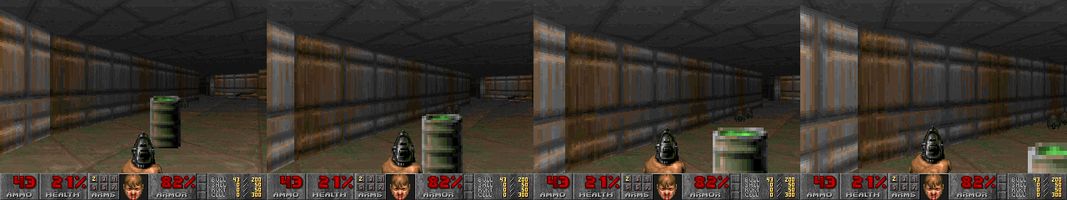
\includegraphics[width=1.0\textwidth]{figures/samples/context_7.png}
    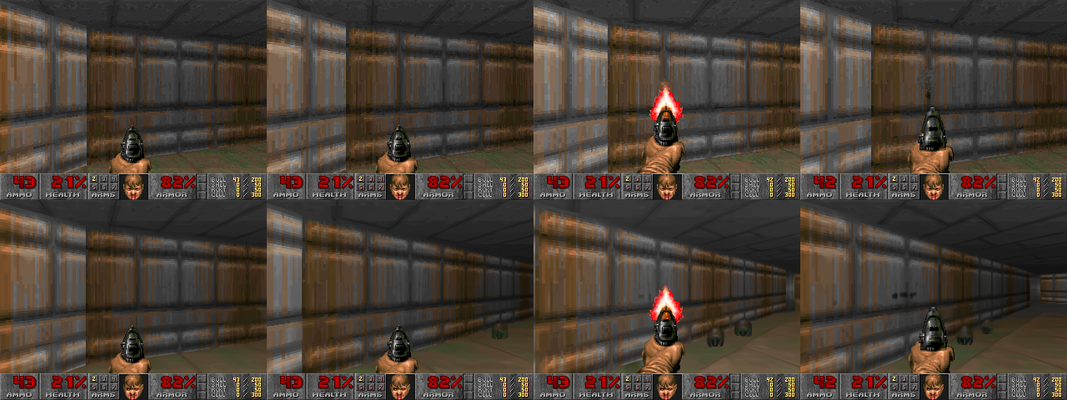
\includegraphics[width=1.0\textwidth]{figures/samples/gt_vs_pred_7.png}
    \caption{\textbf{模拟模型的自回归评估：样本 \#4。} 上行：上下文帧；中行：真实帧；下行：模型预测。}
    \label{fig:samples_4}
\end{figure}

\clearpage

\subsection{微调潜在解码器示例}
\label{appendix:fine-tune-vae}
图~\ref{fig:vae-ft-ablation} 展示微调 VAE 解码器的效果。
\begin{figure}[h]
    \centering
    \vspace{-0.1in}
    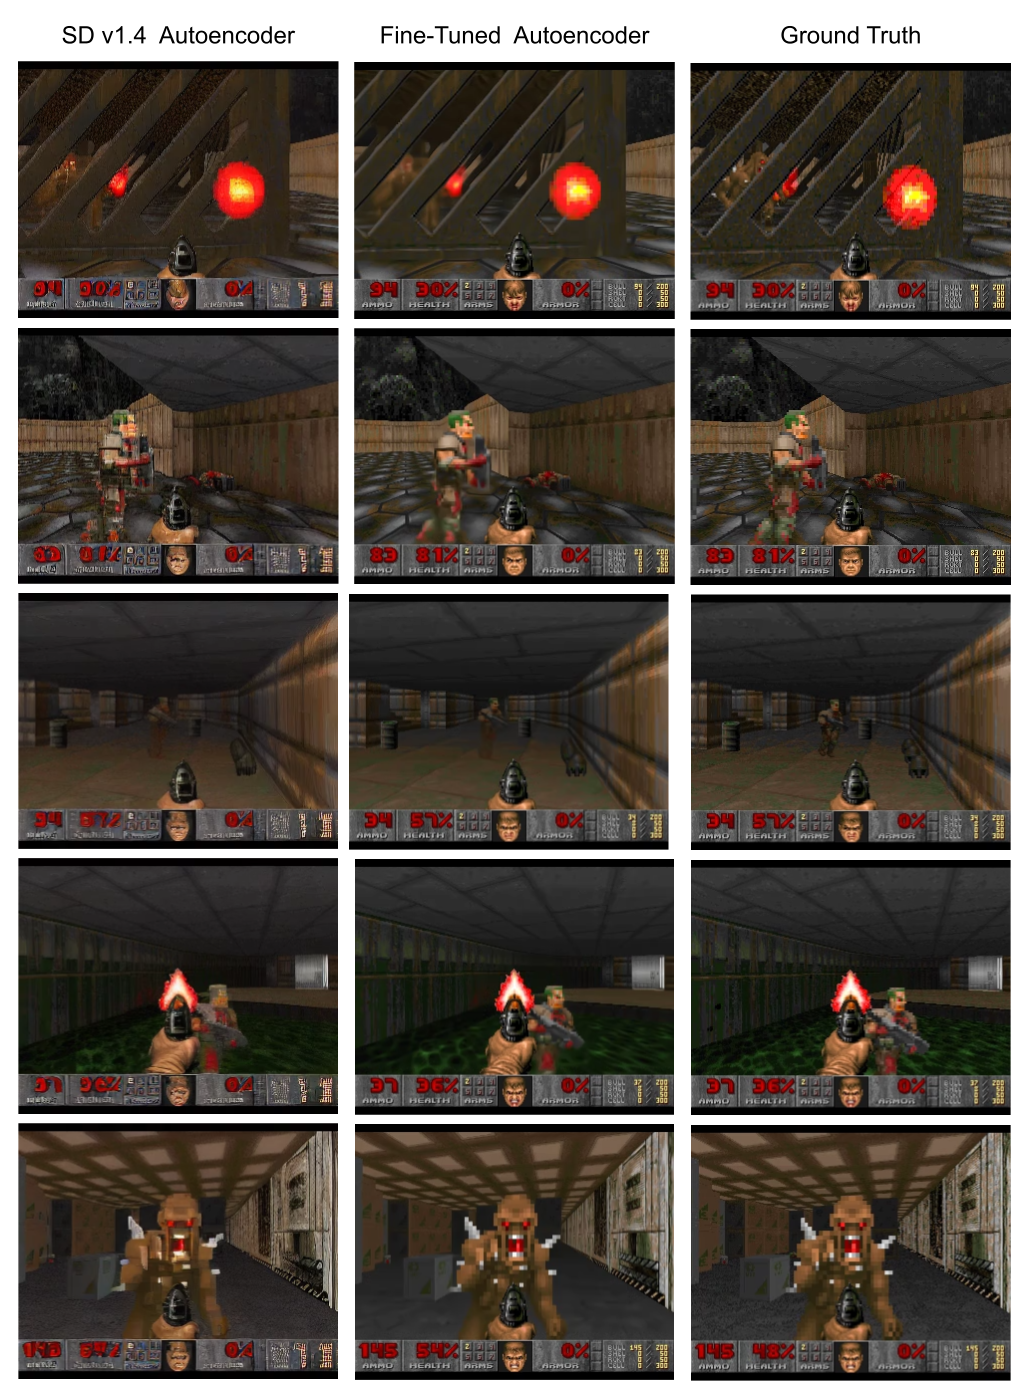
\includegraphics[width=\textwidth]{figures/fine_tuning_autoencoder.png}
    \caption{标准 Stable Diffusion v1.4 潜在解码器（左）、本文微调解码器（中）与真实值（右）的生成对比。冻结解码器会产生明显伪影，例如底部 HUD 数字区域。}
    \label{fig:vae-ft-ablation}
    \vspace{-0.05in}
\end{figure}


\clearpage

\subsection{数据集大小分析}
\label{appendix-dataset-size}
为评估 GameNGen 在不同数据规模下的表现，作者额外训练了只使用 1M、5M 和 10M 样本的模型。图~\ref{fig:dataset_size_psnr} 展示不同数据规模下的 PSNR 曲线。下一帧预测的 PSNR 在包含 2048 条保留轨迹的测试集上评估。结果显示，小数据集上的测试性能更早饱和；而使用 70M 样本时，性能在 700k 训练步后仍持续提升。作为定性评估，作者还用 1M 和 10M 样本模型录制了人类游玩视频；每个模型使用测试集损失最低的 checkpoint（见补充材料中的 \texttt{condition\{1,2\}\_\{1M,10M\}\_examples.mp4}）。1M 样本模型可以渲染新视角，但一致性和游戏逻辑较弱，例如不能正确击杀怪物；10M 样本模型在细节和一致性上有所改善。


\begin{figure}[t]
    \centering
    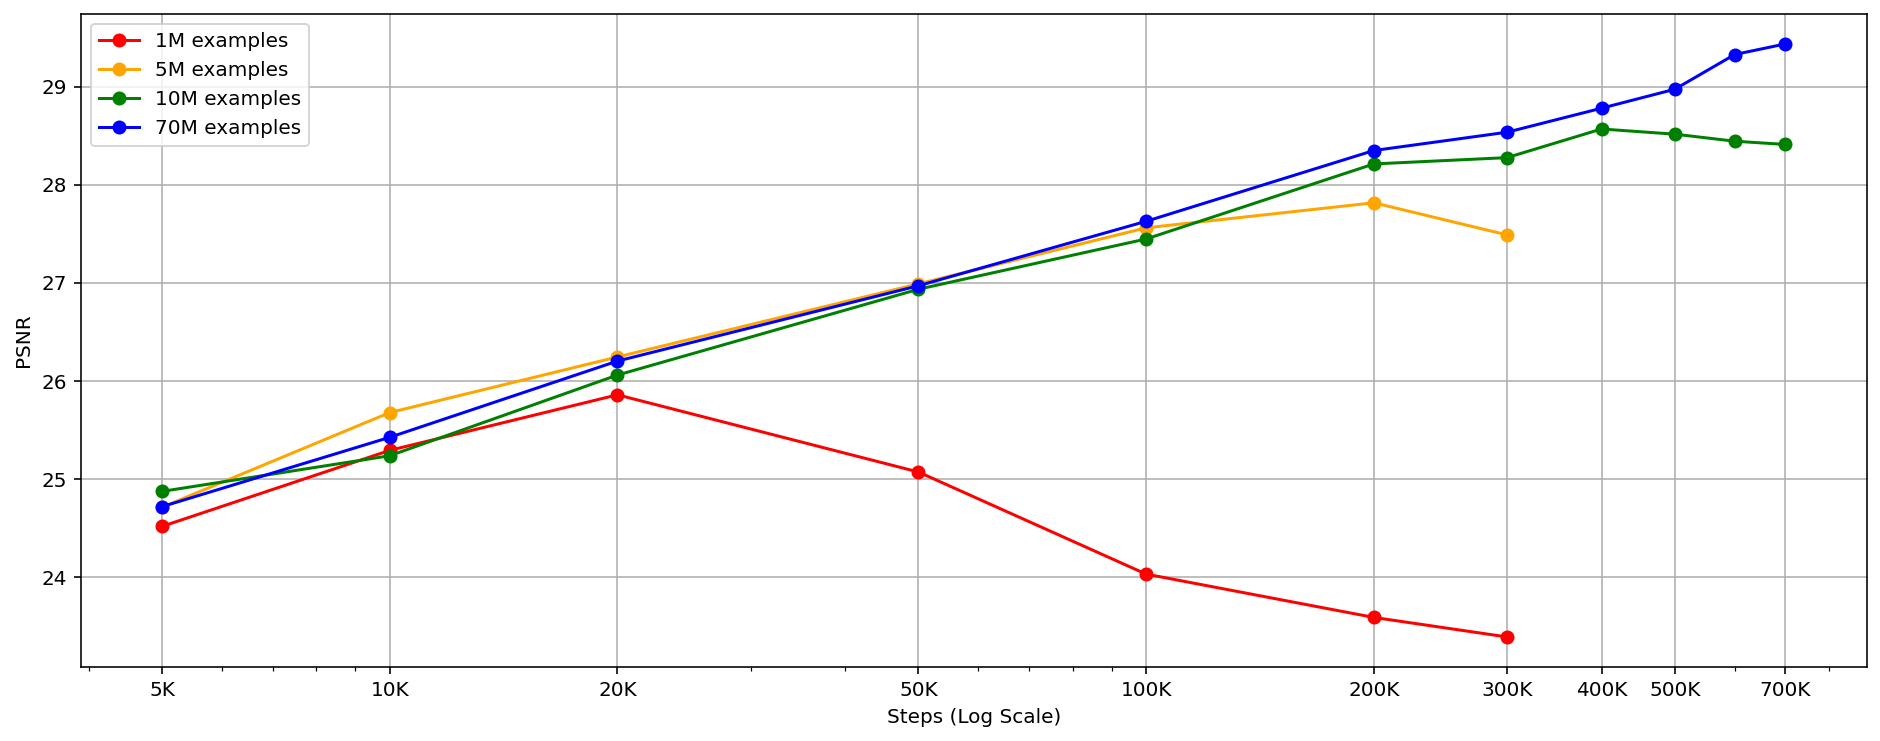
\includegraphics[width=1.0\textwidth]{figures/psnr_train_step_curves.png}
    \caption{\textbf{数据集规模影响。} 不同数据规模（1M、5M、10M、70M 样本）下 PSNR 随训练步数变化的曲线，在 2048 条保留测试轨迹上评估。注意，batch size 为 128 时，10k 步略多于 1M 个训练样本。}
    \label{fig:dataset_size_psnr}
\end{figure}

\subsection{分布外采样}
\label{appendix-out-of-distribution}
为进一步探索 GameNGen 生成训练数据中未出现行为的能力，作者从游戏中抽取帧，用图像编辑器手动修改，然后从编辑后的帧开始生成。具体做法是将同一帧复制到整个历史缓冲区，并使用“无按键”动作。为鼓励泛化，在该设置下作者训练了一个新的 GameNGen 模型，并随机化智能体起始位置。由于噪声增强（第~\ref{sec:mitigating ar noise} 节）会使小的局部修改被忽略，作者主要执行更显著的编辑。结果显示，模型通常可以生成训练数据中没有出现过的关卡和情形。
例如，图~\ref{fig:gamengen_edit_monsters} 展示了将一个训练数据中未出现在该区域的游戏角色粘贴到画面中的例子，例如把高级关卡中的怪物插入早期关卡。模型经常能将新增角色一致地整合到新位置，使其移动、向玩家射击并造成伤害。图~\ref{fig:gamengen_edit_structure} 展示了通过插入来自其他区域的墙、门或池塘等元素来修改关卡布局；模型能够将这些元素整合进环境，并在玩家移动时渲染新的视角。作者将这些初步结果留待后续进一步研究。


\begin{figure}[t] \centering \includegraphics[width=1.0\textwidth]{figures/gamengen_edit_monsters.pdf} \caption{\textbf{添加角色。} 从包含其他区域角色的手动编辑状态开始生成时，GameNGen 产生的帧。}
\label{fig:gamengen_edit_monsters}
\end{figure}

\begin{figure}[t] \centering \includegraphics[width=1.0\textwidth]{figures/gamengen_edit_structure.pdf} \caption{\textbf{改变结构。} 从手动编辑状态开始生成时，GameNGen 产生的帧；该状态组合了训练数据中没有共同出现过的不同关卡布局特征。} \label{fig:gamengen_edit_structure}
\end{figure}


\newpage
\clearpage
\subsection{奖励函数}
\label{appendix:reward}

RL 智能体的奖励函数是本文方法中唯一针对 DOOM 专门设计的部分，由下列项加和得到：

\begin{enumerate}
    \item 玩家受击：$-100$。
    \item 玩家死亡：$-5000$。
    \item 击中敌人：$300$。
    \item 击杀敌人：$1000$。
    \item 拾取物品或武器：$100$。
    \item 发现隐藏区域：$500$。
    \item 探索新区域：$20 \times (1 + 0.5 \times L_1\text{距离})$。
    \item 生命值变化：$10 \times \Delta$。
    \item 护甲变化：$10 \times \Delta$。
    \item 弹药变化：$10 \times \max(0,\Delta) + \min(0,\Delta)$。
\end{enumerate}

此外，为鼓励智能体产生更平滑、更接近人类的游玩轨迹，每个智能体动作会持续应用 4 帧，并人为提高重复上一动作的概率。

\subsection{减少推理步骤}
\label{appendix:distillation}
作者在不同采样步数下评估 GameNGen 性能。评估使用 35 FPS 数据，以 teacher forcing 轨迹生成 2048 帧；35 FPS 是 ViZDoom 允许的最高采样率，低于模型本身可达到的最高速率。结果显示，将采样步数降至 4 步不会使质量退化；只有使用单步采样时质量才明显下降（见表~\ref{table:diffusion_steps_quality}）。

作为补救，作者参考~\cite{wang2023prolificdreamer} 和~\cite{yin2024onestep} 尝试蒸馏模型。蒸馏训练使用 3 个 U-Net，均由 GameNGen 初始化：生成器、教师和 fake score model。教师在训练中保持冻结；fake score model 持续训练，用标准扩散损失预测生成器输出。训练生成器时，教师和 fake score model 分别预测输入图像中的噪声 $\epsilon_{\text{real}}$ 和 $\epsilon_{\text{fake}}$，然后优化生成器权重，以最小化按像素加权的生成器梯度，即 $\epsilon_{\text{real}} - \epsilon_{\text{fake}}$。蒸馏时，作者使用 CFG=1.5 生成 $\epsilon_{\text{real}}$，训练 1000 步，batch size 为 128。与~\cite{yin2024onestep} 不同，本文在不同噪声水平下训练，且不使用正则化损失。蒸馏显著提升了一步模型质量（见表~\ref{table:diffusion_steps_quality} 中的 “D”），使游戏可以 50 FPS 运行，但仍带来轻微质量损失。

\label{appendix:ablate num sampling steps}

\pagebreak

\subsection{智能体 vs 随机策略}
\label{appendix:agent v random}

图~\ref{fig:agent v random} 展示了在人类短时游玩片段上，自回归生成 3 秒后，使用 RL 智能体数据训练的模型和使用随机策略数据训练的模型相对于真实值的 PSNR。结果显示，智能体数据有时与随机策略相当，有时明显更好。

\begin{figure}[ht]
    \centering
    \vspace{-0.1in}
    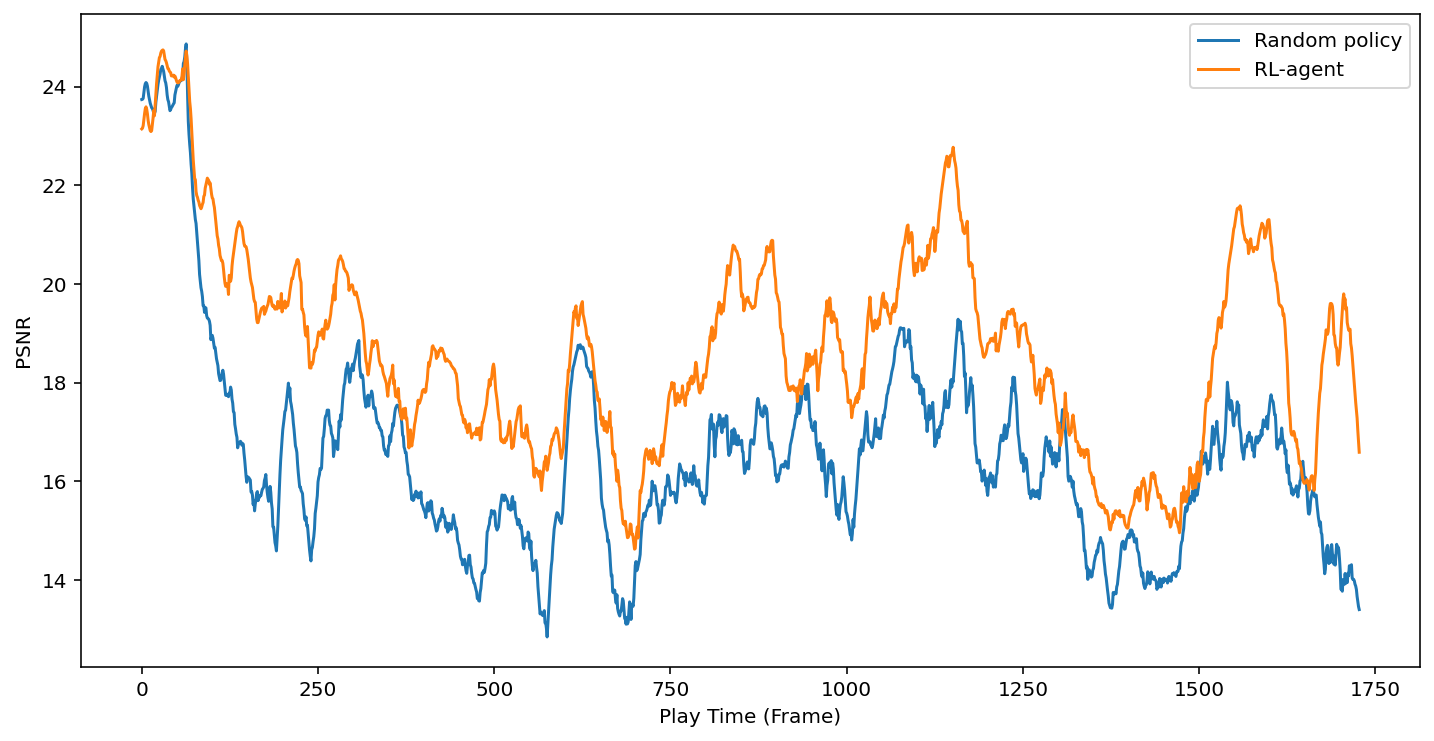
\includegraphics[width=\textwidth]{figures/psnr_over_trajectory.png}
    \caption{\textbf{短时人类游玩中的 RL 智能体数据与随机策略数据对比。} 自回归生成 3 秒后，比较智能体数据模型（橙色）和随机策略数据模型（蓝色）生成帧相对真实值的 PSNR。曲线使用 EMA 平滑，系数为 0.05。}
    \label{fig:agent v random}
    \vspace{-0.05in}
\end{figure}

\subsection{人类评估工具}
\label{appendix:human eval}

图~\ref{fig:eval tool} 展示用于人类评估的工具截图（见第~\ref{sec:sim quality} 节）。
\begin{figure}[ht]
    \centering
    \vspace{-0.1in}
    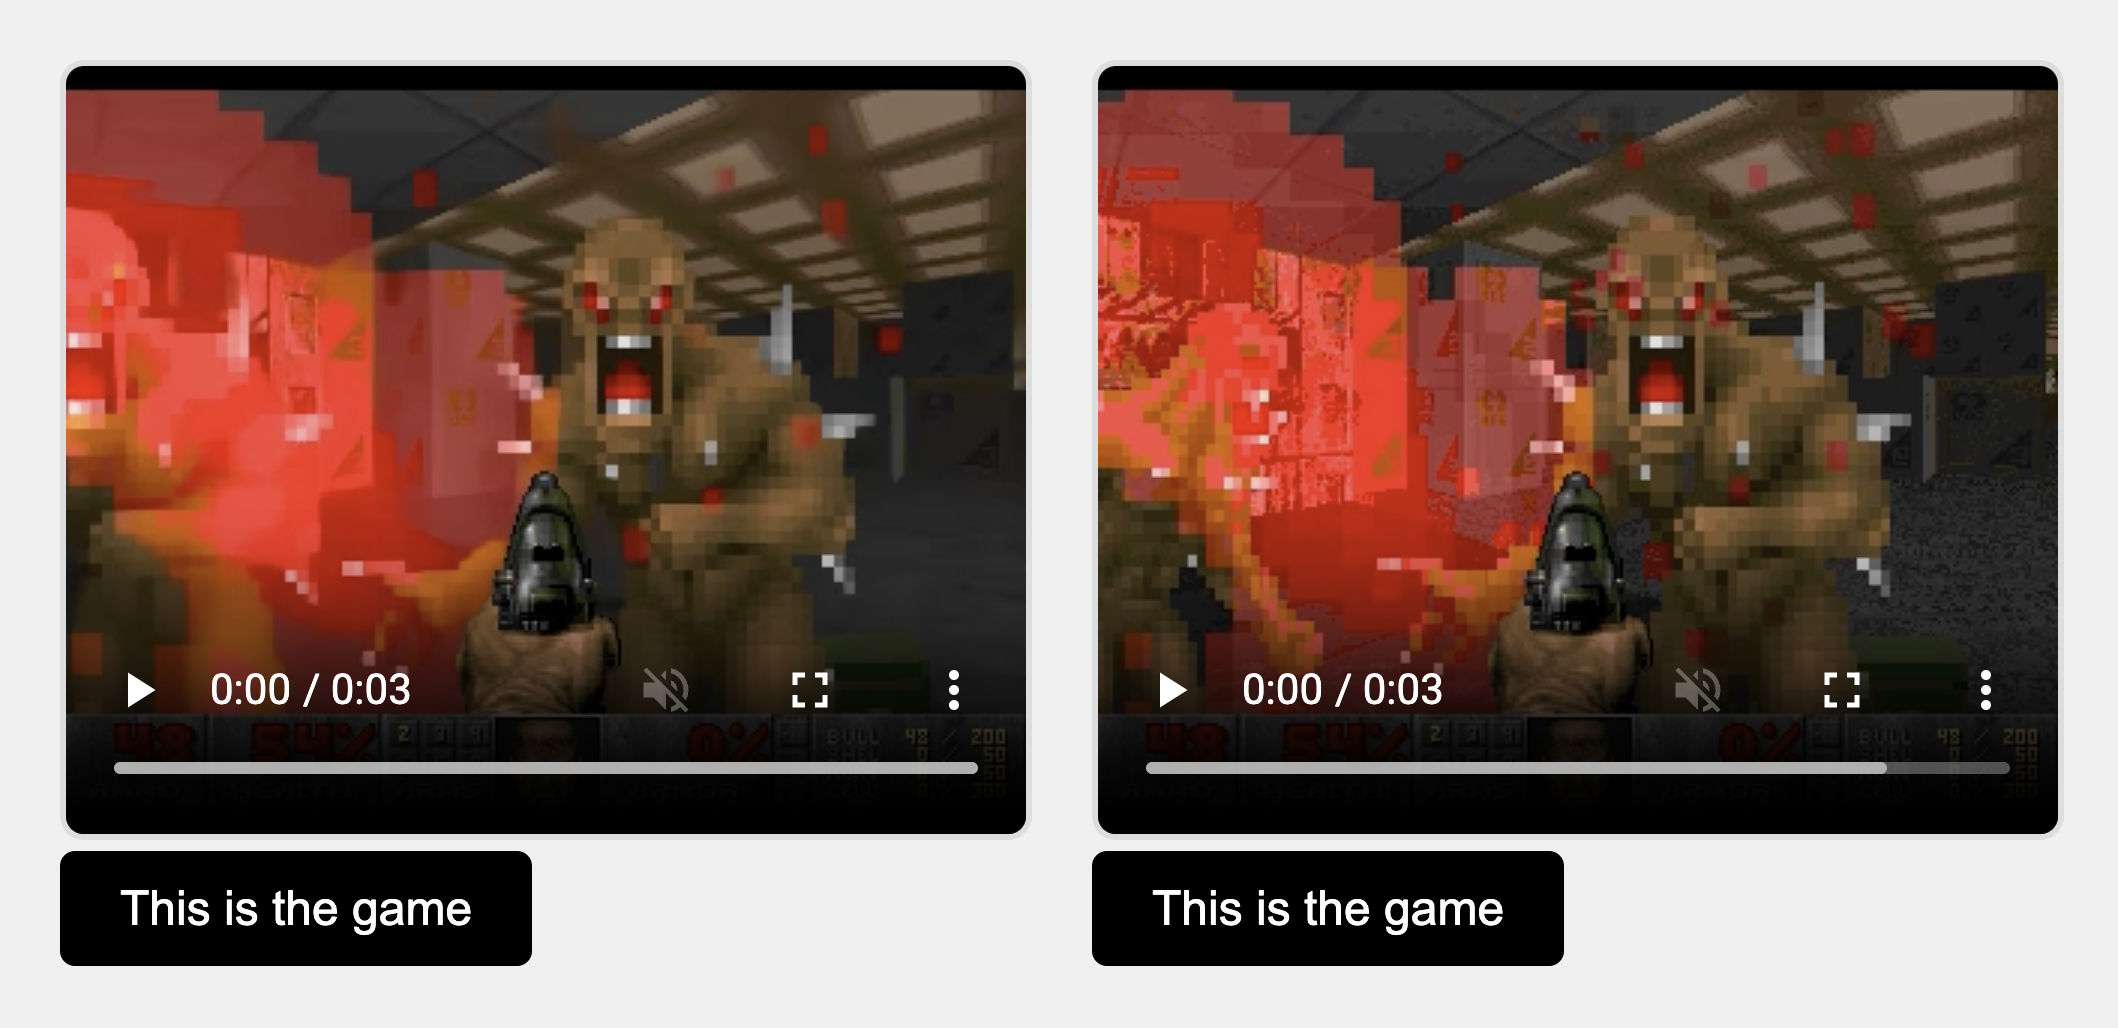
\includegraphics[width=\textwidth]{figures/eval_tool.png}
    \caption{人类评估工具截图（见第~\ref{sec:sim quality} 节）。}
    \label{fig:eval tool}
    \vspace{-0.05in}
\end{figure}

\pagebreak


\subsection{其他相关工作}
\textbf{交互式 3D 模拟。} 计算机图形学已经较成熟地发展了交互式 2D 和 3D 模拟~\citep{realtimerendering}。Unreal 和 Unity 等游戏引擎根据用户输入跟踪世界状态（例如玩家位置、对象和光照）以及游戏逻辑（例如得分），并生成图像流。电影制作常使用计算量较大的光线追踪~\citep{shirley2008realistic}；游戏引擎则优先保证速度，通常以 30 到 60 FPS 运行，并依赖 GPU 优化的多边形光栅化。阴影和光照等物理效果多采用高效近似，而不是完全精确模拟。

\textbf{神经 3D 模拟。} 近年用于重建 3D 表示的神经方法取得了进展。\citep{mildenhall2020nerf} 用深度神经网络参数化辐射场，并针对由多视角图像构成的特定场景进行优化；训练后可以用体渲染采样场景新视角。3D Gaussian Splatting~\citep{kerbl3Dgaussians} 基于 NeRF 思路，但使用 3D Gaussians 和定制光栅化表示场景，从而加速训练和渲染。这些方法能得到较好的重建结果并支持实时交互，但通常局限于静态场景。

\textbf{视频扩散模型。} 扩散模型在文本到图像生成方面取得了很强结果~\citep{saharia2022photorealistic, rombach2022high, ramesh2022hierarchical, podell2023sdxl}，也被用于文本到视频生成~\citep{Ho2022ImagenVH, blattmann2023alignlatentshighresolutionvideo, blattmann2023stablevideodiffusionscaling, gupta2023photorealisticvideogenerationdiffusion, girdhar2023emuvideofactorizingtexttovideo, bartal2024lumierespacetimediffusionmodel}。尽管这些模型在真实感、文本一致性和时间一致性方面已有进展，但对实时应用仍然太慢。本文将这一方向扩展到实时生成，并以历史观测和动作作为条件。

\subsection{模拟平台游戏}

作者还在简单平台游戏 “Chrome Dino” 上进行了实验，以展示 GameNGen 模拟不同游戏类型的能力（见图~\ref{fig:chrome_dino}）。为收集数据，作者使用带经验回放的深度 Q 网络（DQN~\cite{DQN}）训练一个 RL 智能体，奖励函数来自游戏分数。智能体按 epsilon-greedy 策略选择动作，衰减系数为 0.9995。训练期间录制了 2k 个 episode，并用主文相同设置训练扩散模型，改动包括：(1) 使用 32 帧上下文，(2) 分辨率为 $256\times512$，(3) 只训练 3000 步。与 DOOM 类似，GameNGen 生成的模拟可以在长轨迹上实时游玩，视觉质量接近源游戏（示例视频见补充材料）。

此外，GameNGen 还能模拟游戏会话管理动作，例如游戏结束和自动重新开始。为实现这一点，作者将两个随机 episode 拼接，并从拼接序列中抽取 32 帧。若采样上下文跨越两个 episode，模型就能学习会话之间的过渡。

\begin{figure}[ht] \centering 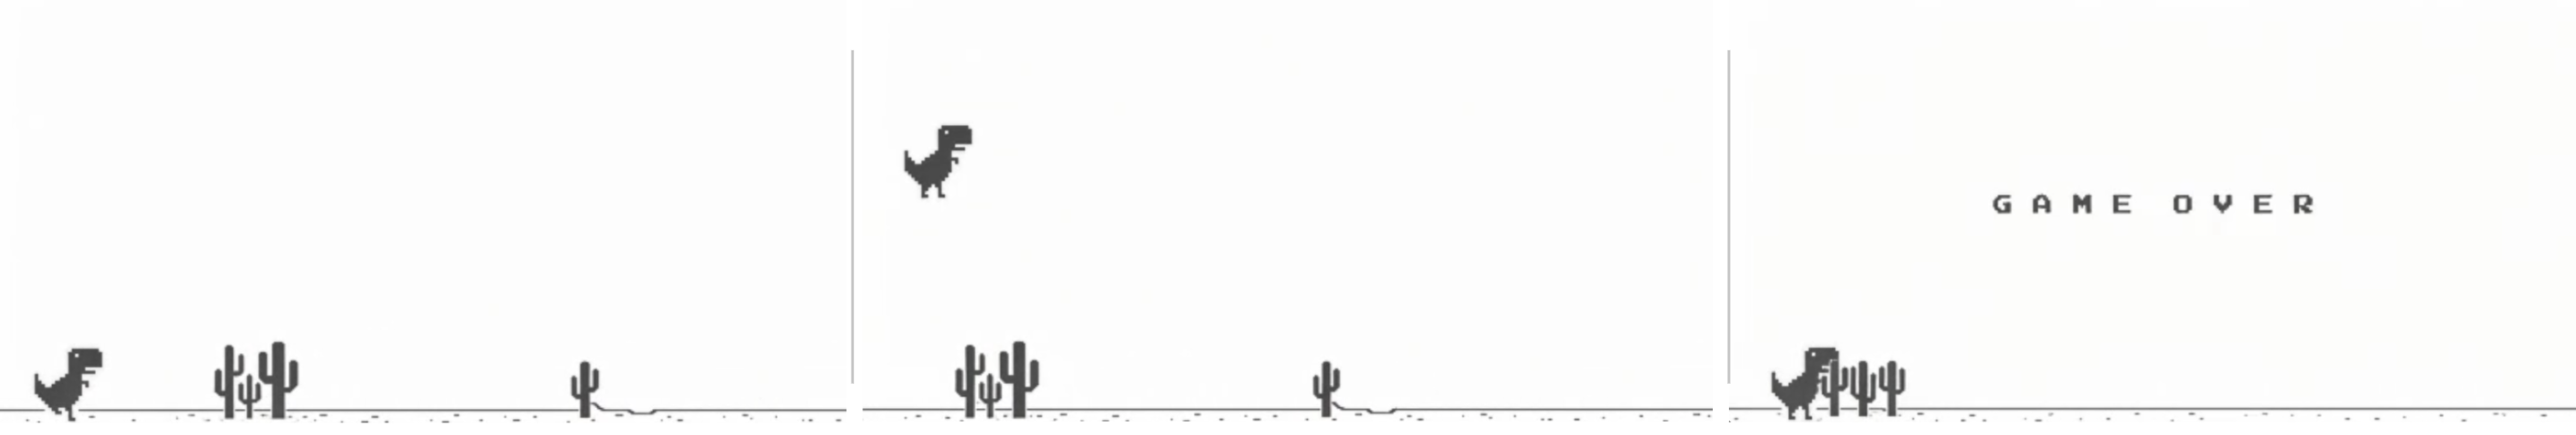
\includegraphics[width=1.0\textwidth]{figures/samples/dino-3.png} \caption{\textbf{“Chrome Dino” 模拟。} GameNGen 在游戏会话结束后自动重启。} \label{fig:chrome_dino}
\end{figure}




\end{document}


